
%----------------------------------------------------------------------------------------
%	PACKAGES AND THEMES
%----------------------------------------------------------------------------------------
\documentclass[t,aspectratio=169,11pt,presentation]{beamer}
%\documentclass[t,aspectratio=169,11pt,presentation]{beamer}
%\documentclass[t,aspectratio=169,11pt,draft]{beamer}


% Define colors
\definecolor{ptb5}{RGB}{54,75,154}	 % NT                   
\definecolor{ptb4}{RGB}{74,123,183} % RC + NT	                    
\definecolor{ptb3}{RGB}{110,166,205}                     
\definecolor{ptb2}{RGB}{152,202,225}% EC + RC + NT                  
\definecolor{ptb1}{RGB}{194,228,239}
\definecolor{ptg0}{RGB}{234,236,204}
\definecolor{ptr1}{RGB}{254,218,139} %EC only
\definecolor{ptr2}{RGB}{253,179,102}	                    
\definecolor{ptr3}{RGB}{246,126,75} % AT +	EC + RC                    
\definecolor{ptr4}{RGB}{221,61,45}	 % AT + EC                   
\definecolor{ptr5}{RGB}{165,0,38}	 % AT	   

\usetheme{Boadilla}




% Footer and page numbers

% First remove the navigation symbols from the bottom of all slides 
\setbeamertemplate{navigation symbols}{} 

% Remove the colored line at the bottom
\setbeamertemplate{footline}{}


% Customize items
\setbeamertemplate{itemize items}{\color{ptb2}{\rule[0.05em]{0.6em}{0.6em}}}
\setbeamertemplate{itemize subitem}{\color{ptb2}{\raisebox{0.12em}{$\blacktriangleright$}}}
\setbeamercolor{enumerate item}{fg=black}
\setbeamertemplate{enumerate item}[default]
\setbeamercolor{enumerate subitem}{fg=black}
\setbeamertemplate{enumerate subitem}[default]


\setbeamercolor{subsection in toc}{bg=white,fg=black}




% Table of Contents (if we have one)
\setbeamertemplate{section in toc}{\inserttocsectionnumber.~\inserttocsection}
\setbeamercolor{section in toc}{bg=white,fg=black}
\setbeamertemplate{subsection in toc}{%
  \hspace{1.2em}{{\color{ptb5}{\rule[0.05em]{0.6em}{0.6em}}}~\inserttocsubsection\par}
}
\setbeamercolor{subsection in toc}{bg=white,fg=black}


% Customize beamer colors

\setbeamercolor{titlelike}{fg=white,bg=ptb5}
\setbeamercolor{button}{bg=ptb4,fg=white}
%}

% Nicer looking Itemize and enumerate environments
\newenvironment{wideitemize}{\itemize\addtolength{\itemsep}{14pt}}{\enditemize}
\newenvironment{wideenumerate}{\enumerate\addtolength{\itemsep}{14pt}}{\endenumerate}

% Import packages
\usepackage[default]{lato} % More modern looking font than Helvetica
\usepackage{geometry,caption,color,setspace,dsfont,commath,amsmath,amssymb,bm,mathrsfs}
\usepackage[normalem]{ulem}
\usepackage[comma]{natbib}
\usepackage[short]{optidef}
\usepackage{hhline}
\usepackage{array}
\usepackage{booktabs} % Allows the use of \toprule, \midrule and \bottomrule in tables
\usepackage{adjustbox}
\usepackage{graphicx,xcolor,bbm,xcomment}
\usepackage{appendixnumberbeamer}
\usepackage{textcomp}
\usepackage{colortbl}
\usepackage{subcaption} 
\usepackage{tikz}
\usetikzlibrary{calc,patterns,positioning}
\usepackage{pdflscape}
\usepackage{environ}
\usepackage{array}
\usepackage{etoolbox}
\usepackage[normalem]{ulem}
\BeforeBeginEnvironment{itemize}{\par}
\BeforeBeginEnvironment{enumerate}{\par}

\bibliographystyle{ecta}

\newcommand*\diff{\mathop{}\!\mathrm{d}}


% Make Section Header Frames
\AtBeginSection[]{

  \setbeamercolor{titlelike}{bg=ptb5,fg=white}
  \setbeamertemplate{navigation symbols}{} 
  \begin{frame}[noframenumbering]
  \vfill
  \centering
  \begin{beamercolorbox}[sep=8pt,center,shadow=true,rounded=true]{title}
    \usebeamerfont{title}\insertsectionhead\par%
  \end{beamercolorbox}
  \vfill
  \end{frame}
  % Make a new prettier page number
\addtobeamertemplate{navigation symbols}{}{%
    \usebeamerfont{footline}%
    \hspace{5em}%
    {\color{black!50}{\small\insertframenumber/\inserttotalframenumber}}%
}
\setbeamercolor{titlelike}{fg=ptb5,bg=white}
}

\AtBeginSubsection[]{
  \setbeamertemplate{navigation symbols}{} 
  \begin{frame}[noframenumbering]
  \vfill
  \centering
  \begin{beamercolorbox}[sep=8pt,center,shadow=false,rounded=true]{title}
    \usebeamerfont{title} \insertsubsectionhead\par%
  \end{beamercolorbox}
  \vfill
  \end{frame}
  % Make a new prettier page number
\addtobeamertemplate{navigation symbols}{}{%
    \usebeamerfont{footline}%
    \hspace{5em}%
    {\color{black!50}{\small\insertframenumber/\inserttotalframenumber}}%
}
}



\tikzset{
    invisible/.style={opacity=0},
    visible on/.style={alt={#1{}{invisible}}},
    alt/.code args={<#1>#2#3}{%
      \alt<#1>{\pgfkeysalso{#2}}{\pgfkeysalso{#3}} % \pgfkeysalso doesn't change the path
    },
  }
  
  
\makeatletter
\newsavebox{\measure@tikzpicture}
\NewEnviron{scaletikzpicturetowidth}[1]{%
  \def\tikz@width{#1}%
  \def\tikzscale{1}\begin{lrbox}{\measure@tikzpicture}%
  \BODY
  \end{lrbox}%
  \pgfmathparse{#1/\wd\measure@tikzpicture}%
  \edef\tikzscale{\pgfmathresult}%
  \BODY
}
\makeatother

\tikzset{
  pics/student/.style args={#1,#2}{
     code={
       \filldraw [fill=#1,draw=black,visible on=#2] (.05,.15) .. controls (.05,.7) and (.65,.8) .. (.75,.2) .. controls (.55,.05) and (.05,0) .. (.05,.15) ;
       \filldraw [fill=#1,draw=black,visible on=#2] (.35,.75) circle [radius=.22];
     }
  }
}


\title{Recovering Welfare Weights from Socially Inefficient Allocations} 

\author{Tanner Eastmond \hfill \and Nathan Mather    \\   \textit{teastmond@ucsd.edu}\hfill \textit{njmather{\fontfamily{qag}\selectfont @}umich.edu} \\ {\color{white}{t}} \\  Michael D Ricks  \and \hfill  Julian Betts \\
\textit{ricksmi{\fontfamily{qag}\selectfont @}umich.edu} \hfill \textit{jbetts@ucsd.edu}} 
\institute{}
\date{\today} 

\begin{document}

\begin{frame}[noframenumbering]
\titlepage 
\end{frame}

% Make a new prettier page number
\addtobeamertemplate{navigation symbols}{}{%
    \usebeamerfont{footline}%
    \hspace{5em}%
    {\color{black!50}{\small\insertframenumber/\inserttotalframenumber}}%
}

%------------------------------------------------
% What is Value added 
%------------------------------------------------
\begin{frame}{Overview}
\begin{wideitemize}
    
\end{wideitemize}

\end{frame}

%------------------------------------------------
% Why do we care 
%------------------------------------------------
\begin{frame}[c]{Visual Intuition }


\centering
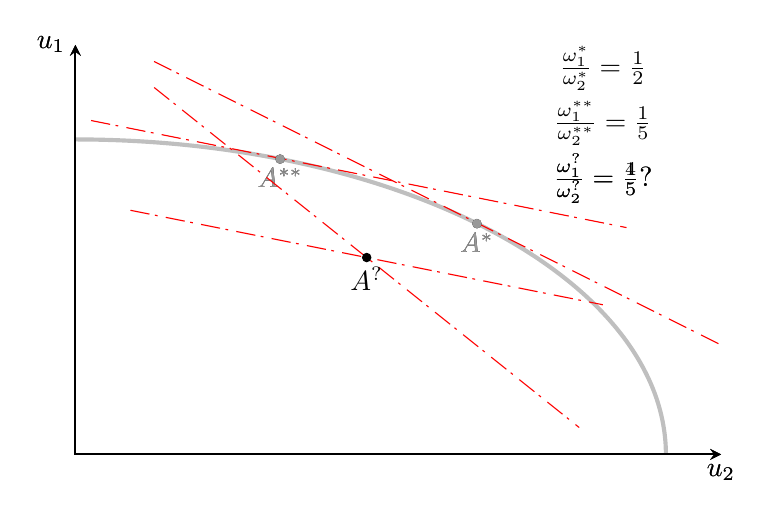
\begin{tikzpicture}
\draw [font=\fontsize{10pt}{10pt}\selectfont,line width=.025cm,stealth-stealth,color=black] (-6.2,5) node [anchor = east] {$u_1$} -- (-6.2, -0.2) -- (2, -.2) node [anchor=north]{$u_2$} ;
\draw [line width=1.5,color=black!25,smooth, samples=100, domain= 0:1] plot({7.5*sin(90*\x)-6.2},{4*cos(90*\x)-.2});

\draw [color=red,dash pattern={on 7pt off 2pt on 1pt off 3pt},smooth, samples=100, domain= -5.2:2,visible on = <3-4>] plot(\x,{-.5*(\x) +2.19});
\filldraw[color=black, fill=black, visible on = <2-4>] (-1.1,2.73) circle (1.5pt) node[font=\fontsize{10pt}{10pt}\selectfont,anchor=north] {$A^{*}$};
\filldraw[color=black!40, fill=black!40, visible on = <5->] (-1.1,2.73) circle (1.5pt) node[font=\fontsize{10pt}{10pt}\selectfont,anchor=north] {$A^{*}$};


\node (A) at (.5,4.7) [font=\fontsize{10pt}{10pt}\selectfont, visible on = <4->] {$\frac{\omega^{*}_1}{\omega^{*}_2}=\frac{1}{2}$};

\draw [color=red,smooth,dash pattern={on 7pt off 2pt on 1pt off 3pt}, samples=100, domain= -6 :.8,visible on = <6-7>] plot(\x,{-.2*(\x) +2.84});
\filldraw[color=black, fill=black, visible on = <5-7>] (-3.6,3.55) circle (1.5pt) node[font=\fontsize{10pt}{10pt}\selectfont,anchor=north] {$A^{**}$};
\filldraw[color=black!40, fill=black!40, visible on = <8->] (-3.6,3.55) circle (1.5pt) node[font=\fontsize{10pt}{10pt}\selectfont,anchor=north] {$A^{**}$};

\node (B) at (.5,4) [font=\fontsize{10pt}{10pt}\selectfont, visible on = <7->] {$\frac{\omega^{**}_1}{\omega^{**}_2}=\frac{1}{5}$};


\draw [color=red,smooth,dash pattern={on 7pt off 2pt on 1pt off 3pt}, samples=100, domain= -5.2 :.2,visible on = <9-10>] plot(\x,{-.8*(\x) +.3});
\draw [color=red,smooth,dash pattern={on 7pt off 2pt on 1pt off 3pt}, samples=100, domain= -5.5 :.5,visible on = <11-12>] plot(\x,{-.2*(\x) +1.8});
\filldraw[color=black, fill=black, visible on = <8->] (-2.5,2.3) circle (1.5pt) node[font=\fontsize{10pt}{10pt}\selectfont,anchor=north] {$A^{?}$};

\node (C) at (.5,3.3) [font=\fontsize{10pt}{10pt}\selectfont, visible on = <10>] {$\frac{\omega_1^?}{\omega_2^?}=\frac{4}{5}$?};
\node (D) at (.5,3.3) [font=\fontsize{10pt}{10pt}\selectfont, visible on = <12>] {$\frac{\omega_1^?}{\omega_2^?}=\frac{1}{5}$?};





\draw [font=\fontsize{10pt}{10pt}\selectfont,line width=.025cm,stealth-stealth,color=black] (-6.2,5) node [anchor = east] {$u_1$} -- (-6.2, -0.2) -- (2, -.2) node [anchor=north]{$u_2$} ;

\end{tikzpicture}


\end{frame}



%------------------------------------------------
% Model 
%------------------------------------------------


\begin{frame}{Ideas}
    \begin{itemize}
        \item Paths for solving A on interior 
        \begin{itemize}
            \item Welfare function is too rigid (needs more bins or other dimensions) 
            \item It's just noise, how do we model noise? 
        \end{itemize}
    \end{itemize}
\end{frame}



\begin{frame}{welfare function too rigid}

\begin{itemize}
    \item How does two bins limit welfare function 
    \item Explain how adding a bin could get us to point A 
    \item A could be from favoring very high or very low 
\end{itemize}    
\end{frame}


\begin{frame}{How do we solve more general functions? }
\begin{itemize}
    \item Plot a bunch and see whats "close" 
    \item try to eliminate possible weights using revealed preferences 
    \begin{itemize}
        \item May be contradictions 
    \end{itemize}
\end{itemize}    
\end{frame}


\begin{frame}{Is this noise? }
\begin{itemize}
   \item Keep the ratio of high to low gains the same? 
   \begin{itemize}
       \item what is origin? 
       \item is it from 0 gains
   \end{itemize}
   
   \item Or, keep ratio of forgone gains the same
   \begin{itemize}
       \item Move up and over to the frontier. The slope connecting those two points defines the tangent for the point on the frontier. 
   \end{itemize}
\end{itemize}    
\end{frame}

%------------------------------------------------
% How do we answer our question?
%------------------------------------------------



\begin{frame}{Model and settup }

\begin{wideitemize}
     \item There is a public program with two (types of) participants
     \item The social planner allocates services subject to technology constraints
     \begin{itemize}
         \item In our setting this is allocating teachers given class compositions and teacher-school contracts
         \item We think this could maybe apply to other settings with public services (e.g., who do you approve for SSI/SSDI, how do you structure Medicaid, etc.)
         \item Obviously with more flexible technology there will always be more gains
     \end{itemize}
     \item If there are multiple individuals of each type the planner is indifferent between them
     \item For whatever reason (information, communication, free-riding) Coasian solutions fail
     \begin{itemize}
         \item 
     \end{itemize}
     

\end{wideitemize}
\end{frame}


\begin{frame}[c]{Solution Concept }


\centering
\begin{tikzpicture}

\draw [line width=1.5,color=black!25,smooth, samples=100, domain= 0:1] plot({7.5*sin(90*\x)-6.2},{4*cos(90*\x)-.2});

\draw [] (-2.5,2.3) -- (-2.5,3.3);
\draw [] (-2.5,2.3) -- (-.32,2.3);


\filldraw[color=black, fill=black] (-2.5,2.3) circle (1.5pt) node[font=\fontsize{10pt}{10pt}\selectfont,anchor=north] {$A^{?}$};






\draw [font=\fontsize{10pt}{10pt}\selectfont,line width=.025cm,stealth-stealth,color=black] (-6.2,5) node [anchor = east] {$u_1$} -- (-6.2, -0.2) -- (2, -.2) node [anchor=north]{$u_2$} ;

\end{tikzpicture}


\end{frame}


\begin{frame}{Bugs and Questions}

\begin{wideitemize}
     \item Why isn't the allocation on the frontier?
     \begin{itemize}
         \item Optimization is complex or costly given information
         \item The technology/PPF is measured with error
         \item There are other dimensions being optimized over  (this one is a problem)
     \end{itemize}
   \item How do we deal with changes in technology?
        \begin{itemize}
         \item Different tech creates very different total utility for the same indifference ratio...
     \end{itemize}
   
   \item What else?
\end{wideitemize}
\end{frame}


%------------------------------------------------

\setbeamertemplate{navigation symbols}{}

\begin{frame}[c,noframenumbering]
\centering
\Huge{\centerline{To Be Continued...}}
\normalsize njmather{\fontfamily{qag}\selectfont @}umich.edu \hspace{2em}
ricksmi{\fontfamily{qag}\selectfont @}umich.edu \hspace{2em} \normalsize teastmond{\fontfamily{qag}\selectfont @}ucsd.edu
\end{frame}

%------------------------------------------------


\begin{frame}[noframenumbering]
\frametitle{References}
\tiny
\bibliography{citations}
\end{frame}


%----------------------------------------------------------------------------------------
%----------------------------------------------------------------------------------------

\appendix


%----------------------------------------------------------------------------------------
%----------------------------------------------------------------------------------------


\begin{frame}[label=methods]{Methods: Overview}

\begin{wideitemize}

\item WLS has both pros and cons:
\begin{itemize}
    \item Intuitive and can estimate both VA heterogeneity and ``welfare added'' % for any welfare function
    \item The three-step procedure is unwieldy and will make inference challenging
    %    Especially given  multiple hypothesis tests we'd need to conduct at each point along the achievement distribution on the same data 
    \item Does it actually work econometrically...? 
    %(is seemingly unrelated regressions invalidated by reweighting in the second stage?)
\end{itemize}

\item We propose two other methods that could estimate heterogeneous VAM:
\begin{itemize}
    \item Conditional quantile regression
    \item Semiparametric index model
\end{itemize}

\end{wideitemize}

\end{frame}


%----------------------------------
% Method two: Quantile Regression
%--------------------------------------
\begin{frame}{Methods: Conditional Quantile Regression}

\begin{wideitemize}

    \item Conditional quantile regressions recover the effect on the $p$th quantile
    
    \item Simpler estimation procedure
    \begin{enumerate}
        \item Estimate the effect of teachers, $D_j$, at each conditional quantile ($p$)
        % There is a tension here about whether we want the Xs to be evaluated at the given quantile or not...
        %\item \color{gray}{or Use Frisch-Waugh-Lovell to partial out mean predictors then estimate effects of teachers on students at the (unconditional) $p$th quantile]?}
        \item Integrate over the effects using desired welfare weights
    \end{enumerate}

    \item Intuitive analogue to VAM methods that residualize out $X_i$ and run VAM on residuals
    
    \item Now the effect of $X_i$ is also being evaluated at the $p$th (conditional) quantile ...
    

\end{wideitemize}
\end{frame}

%----------------------------------
% Method Three: Kernel Regression
%------------------------------------

\begin{frame}{Methods: Semiparametric Index Model}

\begin{wideitemize}

    \item This method flows (most) directly from the SP motivation about weights
    
    \item  Nonparametrically identify teacher $j$'s effects over the achievement distribution
    \begin{itemize}
        \item Estimate $y_i = \sum _j D_j g_j(\beta X_i) +e_i$  by adapting Ichimura's method \citep{ichimura1993semiparametric}
        \item Integrate over the effects using desired welfare weights
    \end{itemize}
    
    \item Intuitive analogue: predict $\hat{y_i}$ then estimate $\mathbb{E}[y_i|\hat{y_i},j=j']$ for each teacher $j'$

    \item Questions/Issues:
    \begin{itemize}
         \item Are there results to estimating subgroup effects?
         \item This will probably only be powered if we pool over years
         \item How do we think about bandwidth selection? 
    \end{itemize}

    %(Also a place to talk about measuring scores in pctle vs $\sigma$?)

\end{wideitemize}

\vfill
\begin{flushleft}

\hyperlink{next}{\beamerbutton{Back}}
\end{flushleft}
\end{frame}

\begin{frame}{Methods: Lowbel 2015}

\begin{wideitemize}
\item Let $W_i = (X_i,D_i)$, then 

\begin{align*}
    Y_i &= \sum_k g_k (w_{ki} u_{ki}) +u_{0i} = \sum _j D_{j(i)} g_j(\beta X_i) +u_{0i} \\
        & \iff g_k = 0 \forall k\leq |X_i| \text{ and } g_k(D_{ki} u_{ki}) = D_{j(i)} g_j(\beta X_i) \forall k>|X_i| 
\end{align*}

\item This will be true if $g_j(0)=0$, $u_{ki}=\beta X_i$, and $u_{ki}\neq 0$, but even if that is possible, I don't think $\beta X$ will ever be uncorrelated with all $D_j$?
\end{wideitemize}


\end{frame}
\end{document}

